%!TEX root = ../../main.tex
\section{Simulation Results}
\label{sec:Simulation Results}
A simulation of the behaviour of a reflection in a diffraction experiment was performed to test the performance of the forward-backward algorithm.
In the simulation, 100 images were recorded in a diffraction experiment where the intensity of a particular reflection was observed twice, once on the 27th image and again on the 76th image with simulated Gaussian noise.
The observed intensities were 71.43 and 40.13 on images 27 and 76 respectively.
The true structure factor amplitude of the reflection is initially 100 and it decays by 1\% after each image is collected (whether it is observed or not).
The forward-backward algorithm is applied where the process function is defined such that the amplitude decays by 1\% for each image and the observation function is defined as in equation \ref{eq:Observation Model}.
The estimate supplied to the forward-backward algorithm for the initial amplitude is 200, double the value of the true value of 100.
The results of the forward-backward algorithm for cycles 1, 2 and 10 are shown in Figure~\ref{fig:forward-backward algorithm simulation results - good}.
\begin{figure}
	\centering
    \begin{subfigure}[b]{1.0\textwidth}
        \centering
        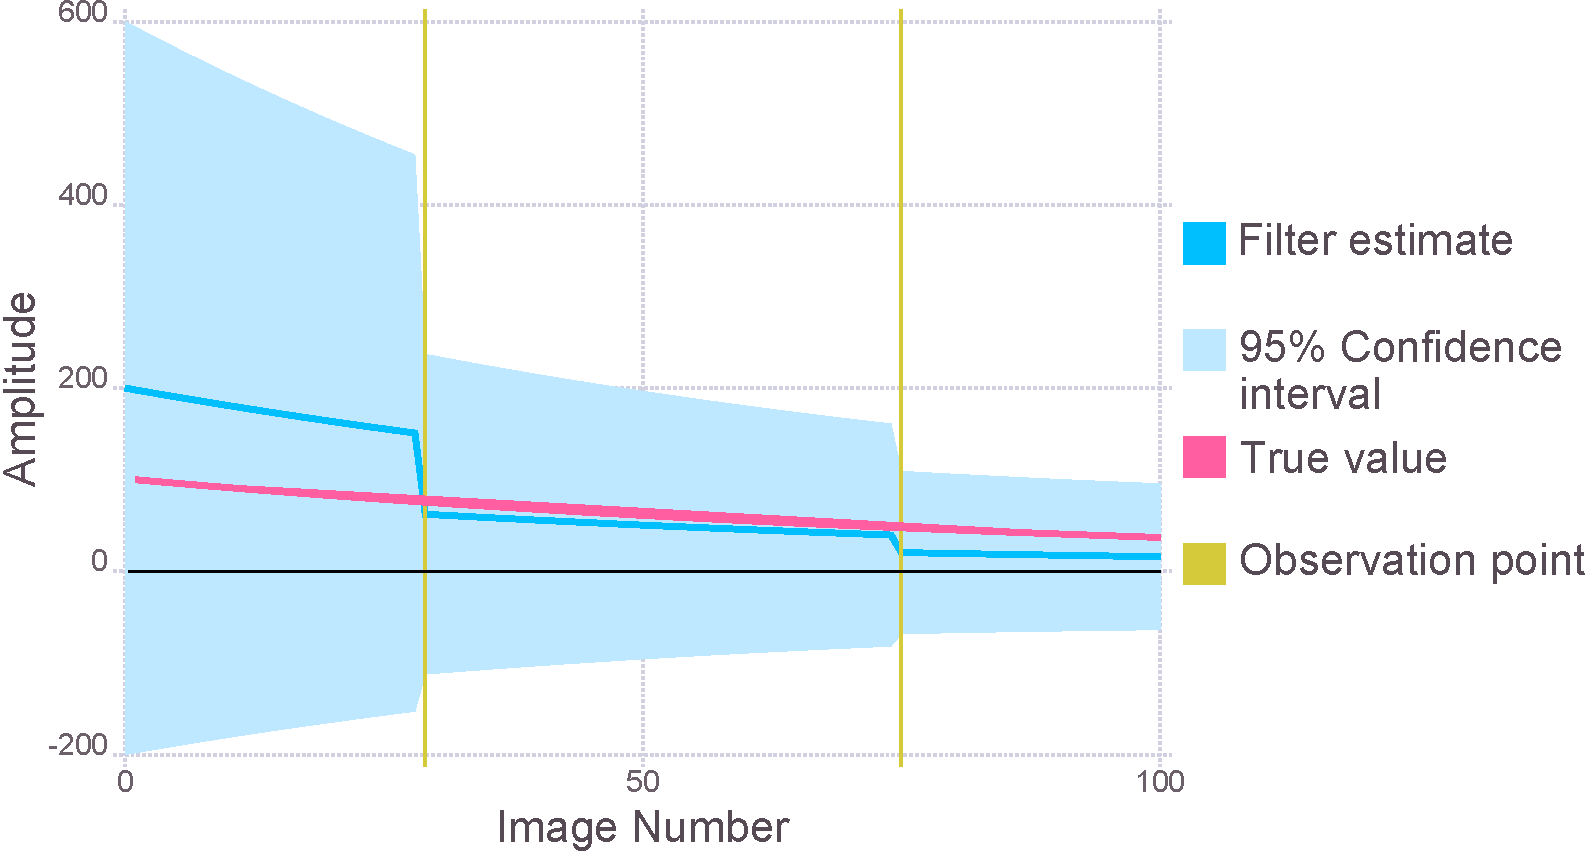
\includegraphics[width=\textwidth]{figures/datared/intDecSim_Filt1.pdf}
        \caption{Cycle 1: forward pass.}
        \label{fig:UKF simulation results - cycle 1 - good}
    \end{subfigure}
    \\
	\begin{subfigure}[b]{1.0\textwidth}
        \centering
        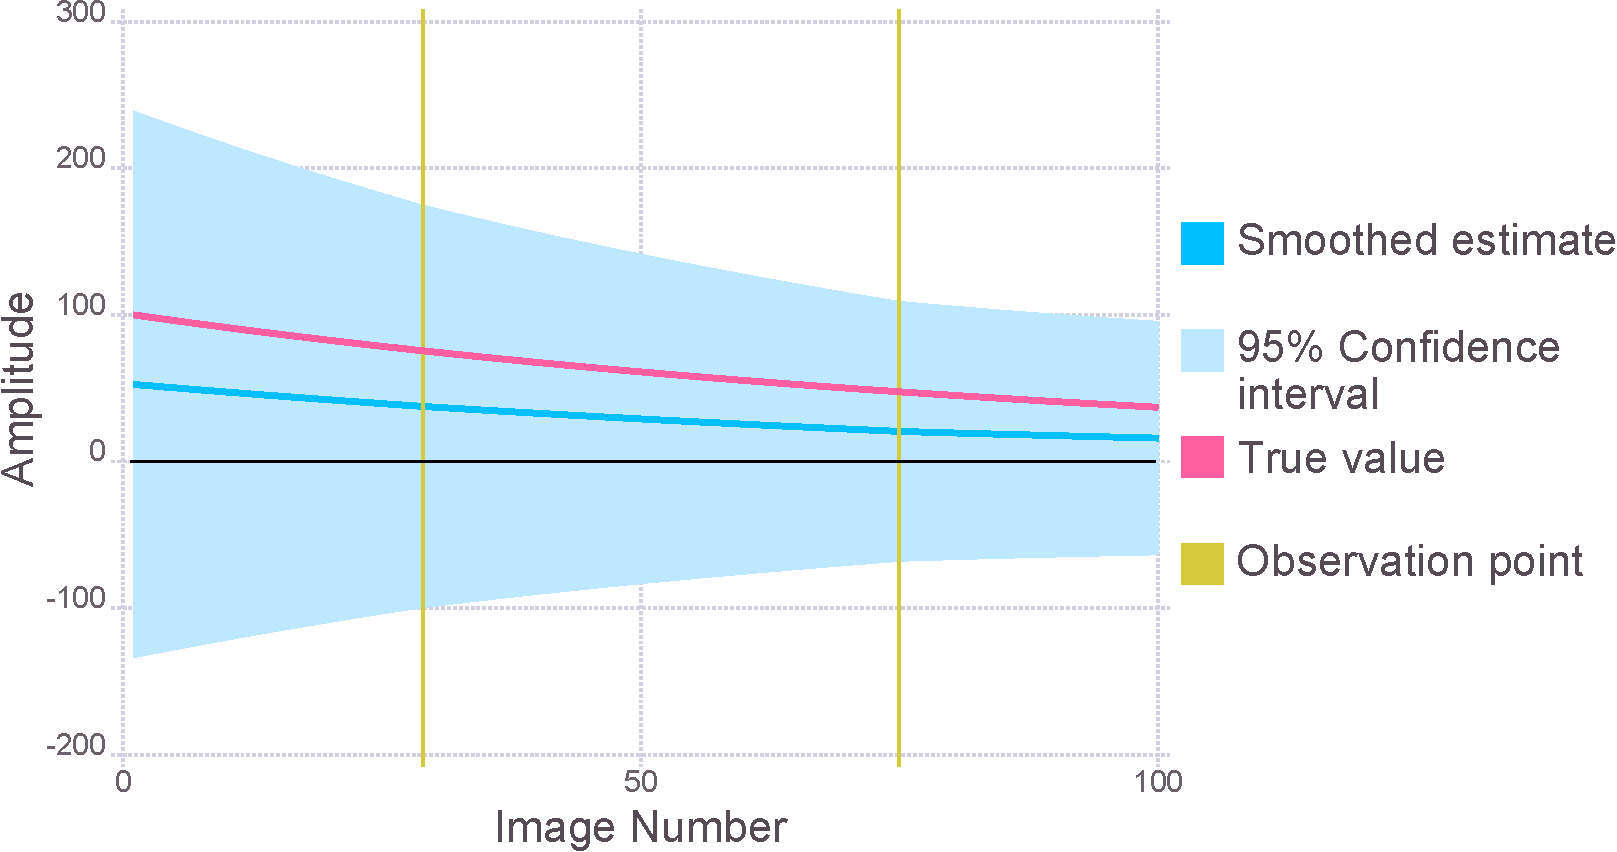
\includegraphics[width=\textwidth]{figures/datared/intDecSim1.pdf}
        \caption{Cycle 1: backward pass.}
        \label{fig:URTSS simulation results - cycle 1 - good}
    \end{subfigure}
\end{figure}
\begin{figure}
    \ContinuedFloat
    \begin{subfigure}[b]{1.0\textwidth}
        \centering
        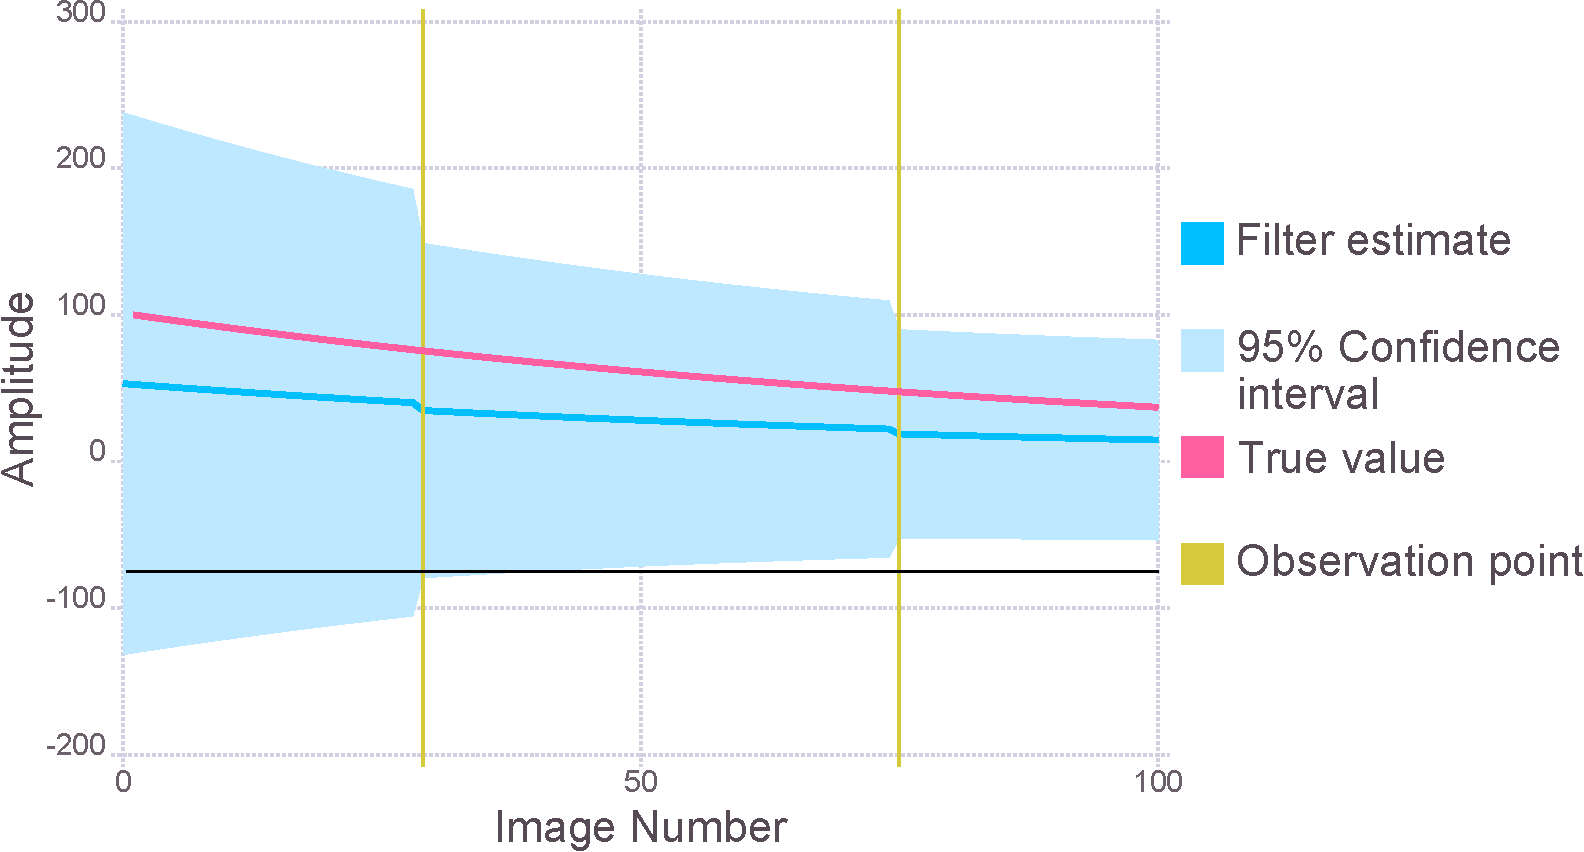
\includegraphics[width=\textwidth]{figures/datared/intDecSim_Filt2.pdf}
        \caption{Cycle 2: forward pass.}
        \label{fig:UKF simulation results - cycle 2 - good}
    \end{subfigure}
    \\
    \begin{subfigure}[b]{1.0\textwidth}
        \centering
        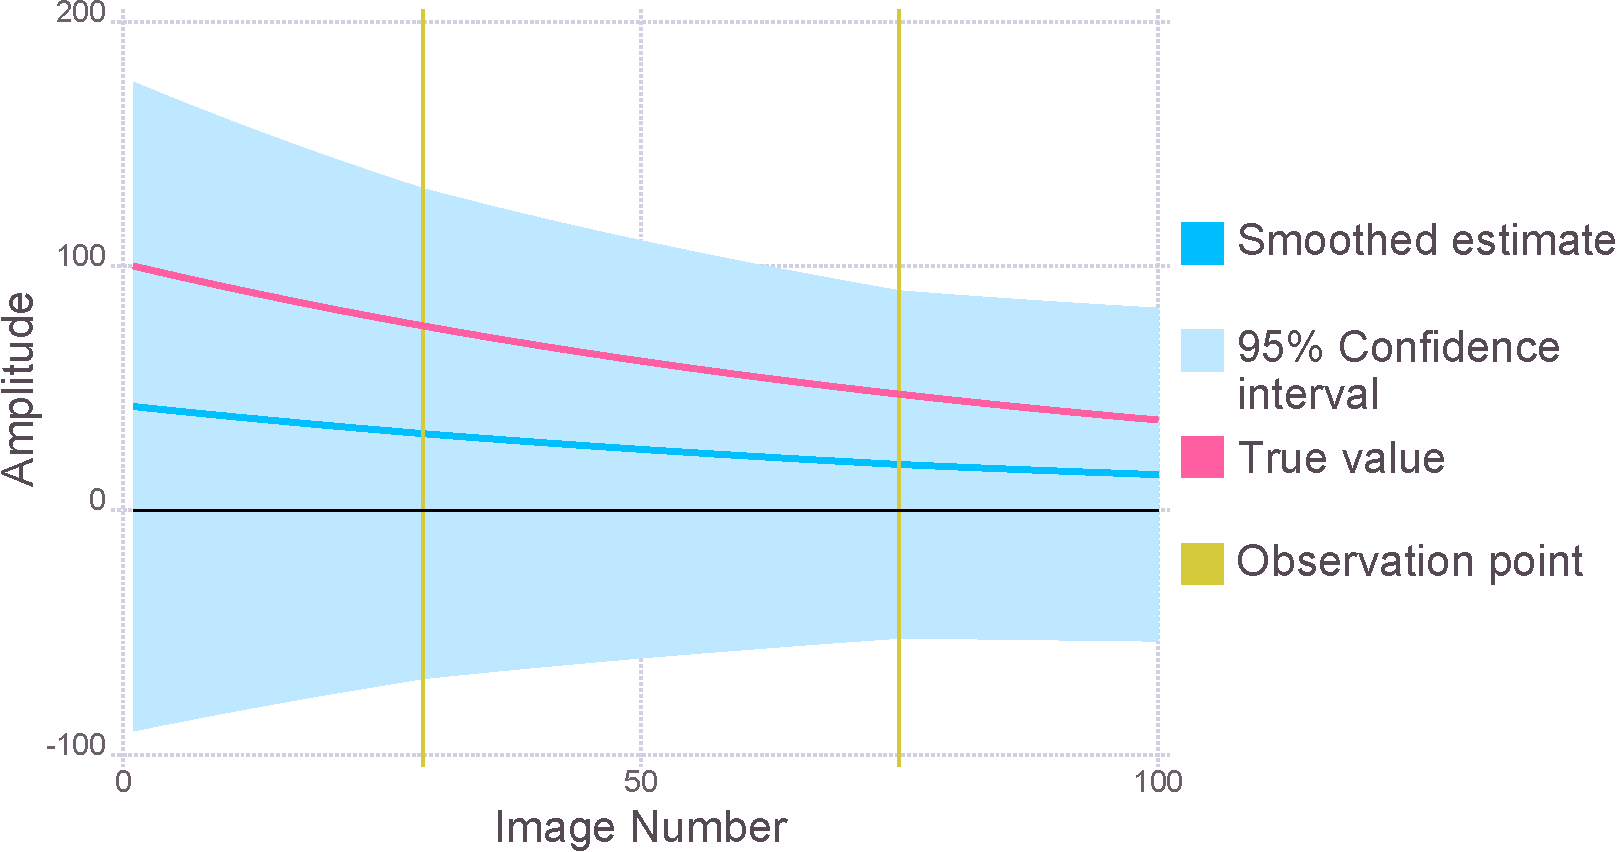
\includegraphics[width=\textwidth]{figures/datared/intDecSim2.pdf}
        \caption{Cycle 2: backward pass.}
        \label{fig:URTSS simulation results - cycle 2 - good}
    \end{subfigure}
\end{figure}
\begin{figure}
    \ContinuedFloat
    \begin{subfigure}[b]{1.0\textwidth}
        \centering
        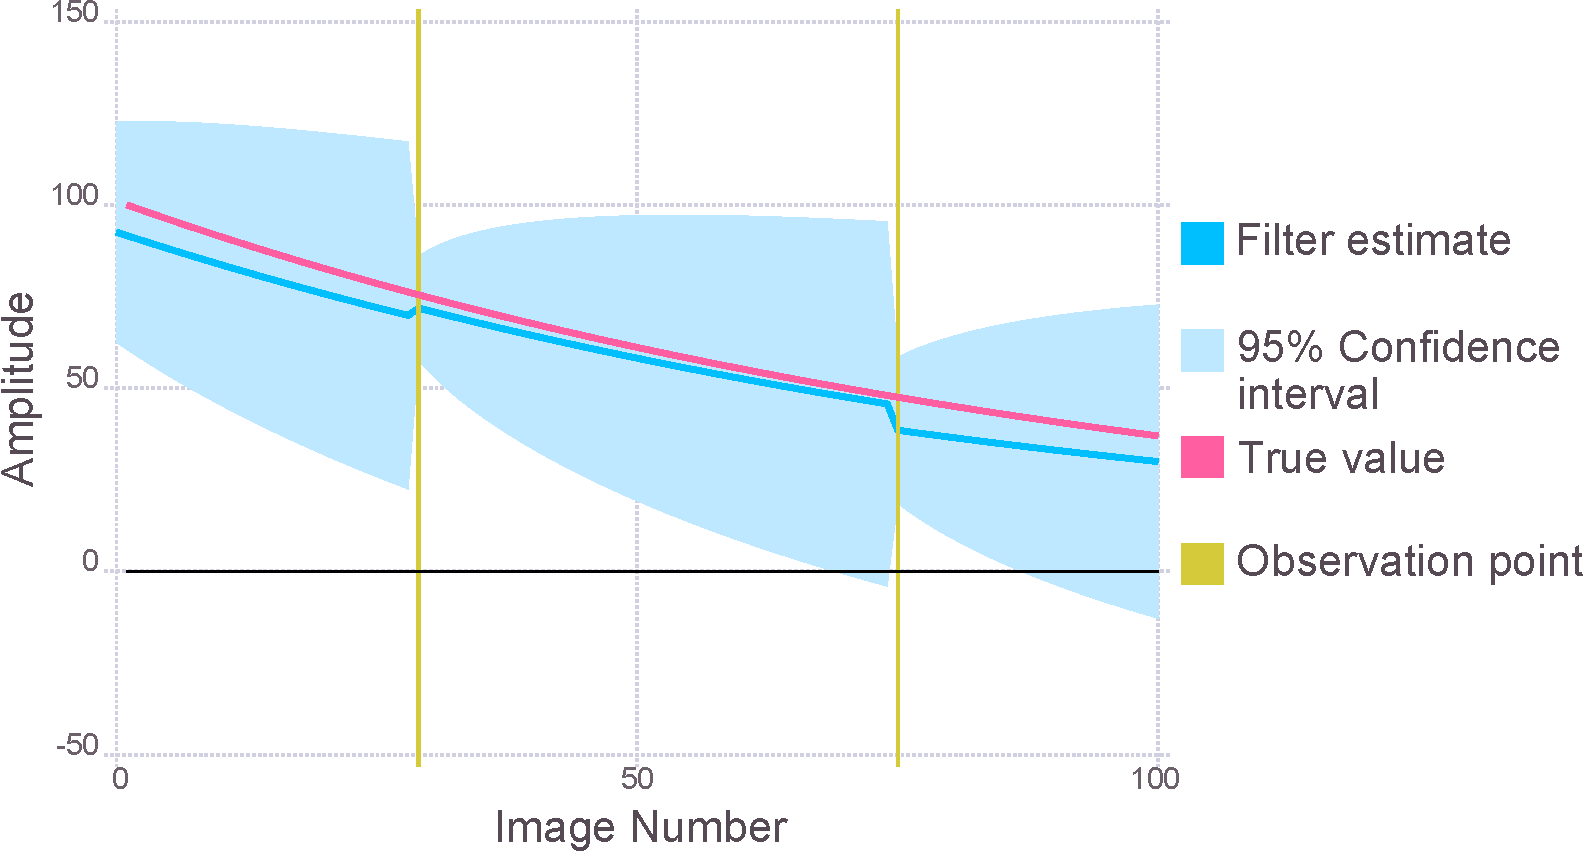
\includegraphics[width=\textwidth]{figures/datared/intDecSim_Filt10.pdf}
        \caption{Cycle 10: forward pass.}
        \label{fig:UKF simulation results - cycle 10 - good}
    \end{subfigure}
    \\
    \begin{subfigure}[b]{1.0\textwidth}
        \centering
        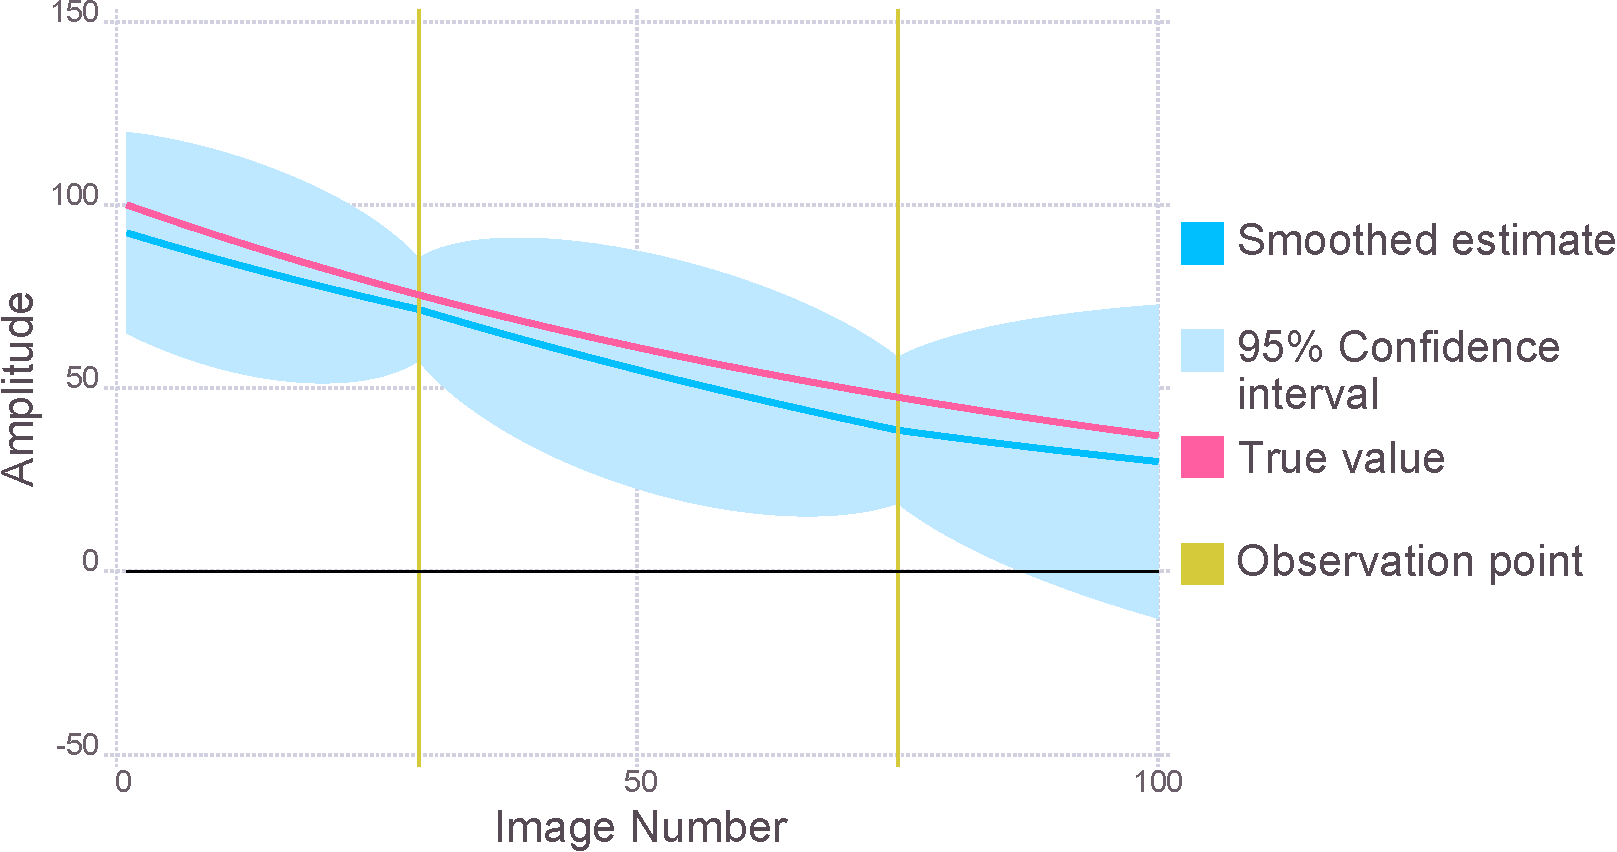
\includegraphics[width=\textwidth]{figures/datared/intDecSim10.pdf}
        \caption{Cycle 10: backward pass.}
        \label{fig:URTSS simulation results - cycle 10 - good}
    \end{subfigure}
    \caption{Forward-backward algorithm results for a simulated reflection observed on image 27 and 76 (solid gold lines) of a dataset consisting of 100 images.
    As the number of cycles increases, the forward-backward estimate (blue solid line) approaches the true value (pink solid line) and the 95\% confidence interval decreases (light blue shaded region).}
    \label{fig:forward-backward algorithm simulation results - good}
\end{figure}

At the very beginning of the algorithm, the filtering estimates (solid blue line Figure~\ref{fig:UKF simulation results - cycle 1 - good}) do not predict the true value (solid pink line) very well.
This is because no observations are made until the 27th image, therefore the estimates propagate according to the defined process function.
At image 27 the first observation is made, represented by the vertical solid gold line, which is when the filtering estimate approaches the amplitude value required to produce the observed intensity according to the observation equation \ref{eq:Observation Model}.
The forward pass continues to propagate the estimates according to the process function until it reaches the second observation and sharply changes value to what it deems optimum.
The smoothing algorithm attempts to consolidate the optimal values found during the forwards pass whilst maximising the probability of the estimate of the state at time i producing the state at time i + 1.
This results in smoother state predictions, as evidenced by the smoother blue solid line in Figure~\ref{fig:URTSS simulation results - cycle 1 - good}, and a reduced overall uncertainty (the light blue shaded region represents the 95\% confidence interval).
The initial value found during the smoothing is also closer to the true value.
The second forward-backward pass shows the same characteristics, whereby the smoother gives a smaller uncertainty estimate and smoothes the values from the filtering pass (Figures~\ref{fig:UKF simulation results - cycle 2 - good} and \ref{fig:URTSS simulation results - cycle 2 - good}).
After 10 forward-backward cycles the smoothed estimates are very close to the true values (Figure~\ref{fig:URTSS simulation results - cycle 10 - good}).
Importantly the uncertainty values are smallest at the points where the observations are made as expected.

The log likelihoods for the 10 cycles, calculated using the natural logarithm of equation \ref{eq:FBA likelihood function}, were also calculated and are shown in Figure~\ref{fig:Simulation Log likelihood - good}.
\begin{figure}[ht!]
    \centering
    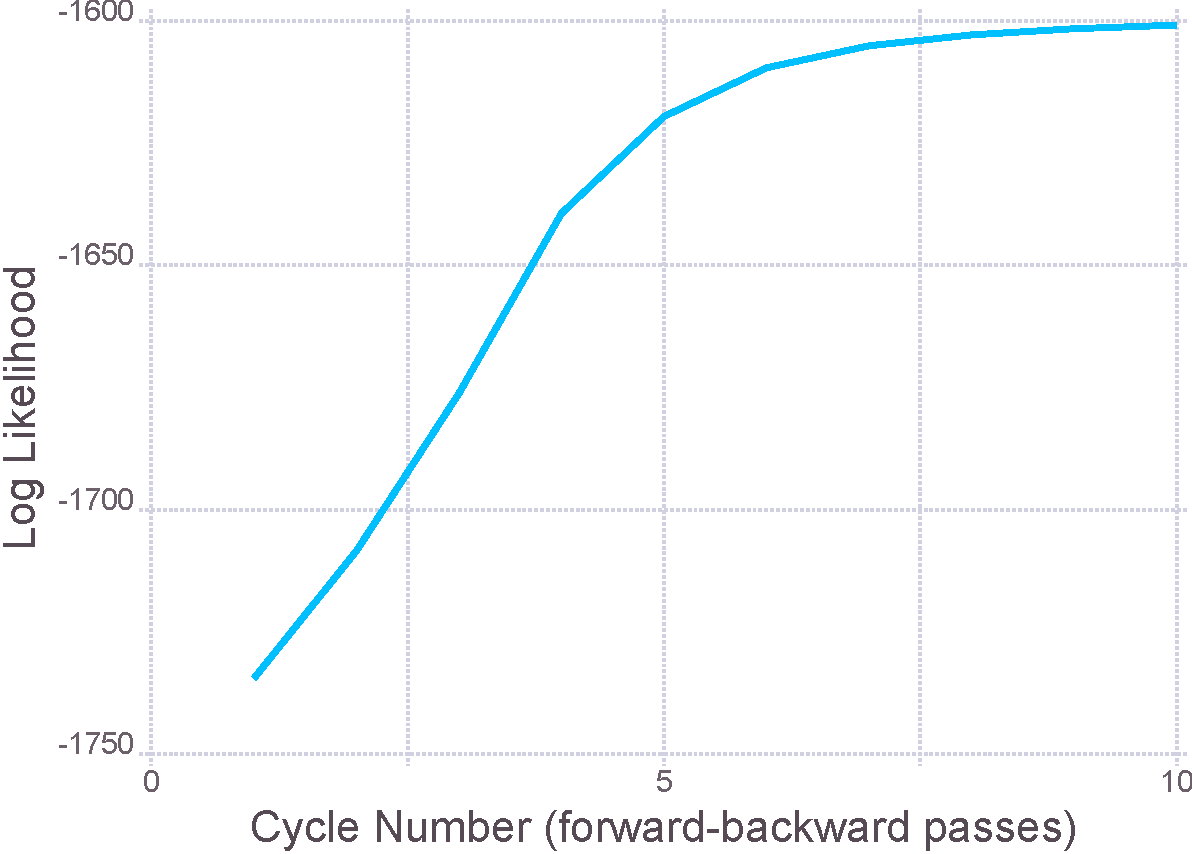
\includegraphics[width=1.0\textwidth]{figures/datared/loglik.pdf}
    \caption{Log likelihood values calculated for each smoothing pass.
    As the cycle number increase the log likelihood starts to plateau meaning that the forward-backward solution is converging on a final solution.}
    \label{fig:Simulation Log likelihood - good}
\end{figure}

It can be seen that as the number of forward-backward passes increases, rate of increase (gradient) tends to zero.
Therefore showing that the smoothed estimates are converging to the optimal solution for the observed data.

\subsection{Weak Data}
\label{sub:Weak Data}
Simulations of the forward-backward algorithm show that the method works very well for strong reflections.
A further simulation was performed to see how effective the algorithm would be for weak reflections.
Again the simulation consisted of 100 images where the intensity of a particular reflection was observed twice, this time on the 41st image and the 99th image with simulated Gaussian noise.
The true structure factor amplitude of this reflection is initially 10 and again decays by 1\% after each image is collected (whether it is observed or not).
The same process and observation functions are defined but the estimate supplied to the forward-backward algorithm for the initial amplitude is 20.
Additive zero-mean Gaussian noise was applied to the observation model to obtain observed intensities of -1.92 and 2.91 on images 41 and 99 respectively.
The results of the forward-backward algorithm for cycles 1 and 8 are shown
\begin{figure}
    \ContinuedFloat
    \begin{subfigure}[b]{1.0\textwidth}
        \centering
        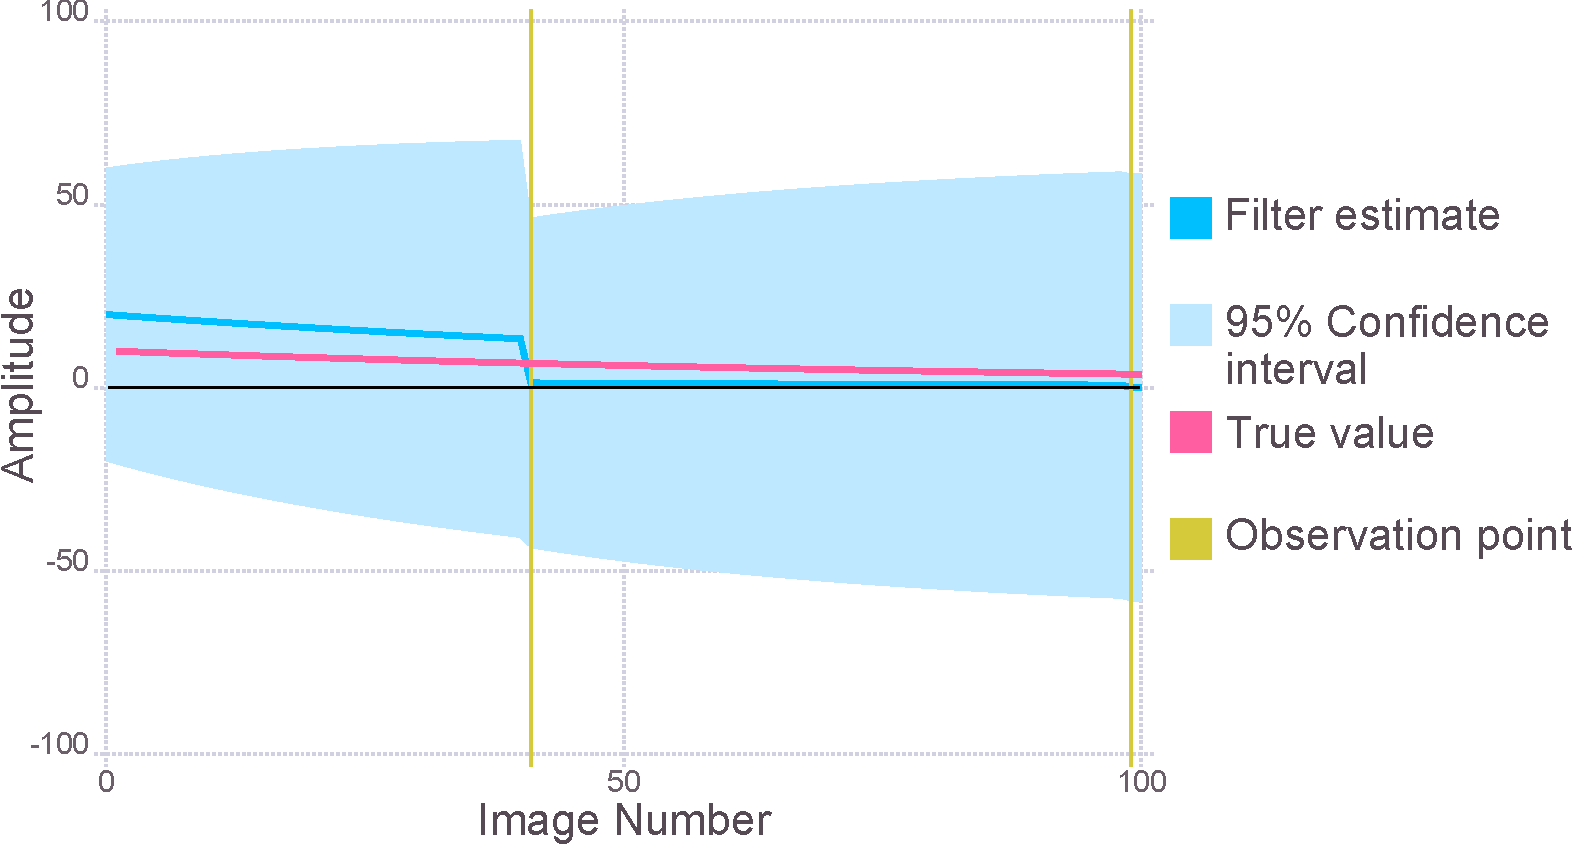
\includegraphics[width=\textwidth]{figures/datared/intDecSim_Filt1_bad.pdf}
        \caption{Cycle 1: forward pass.}
        \label{fig:UKF simulation results - cycle 1 - bad}
    \end{subfigure}
    \\
    \begin{subfigure}[b]{1.0\textwidth}
        \centering
        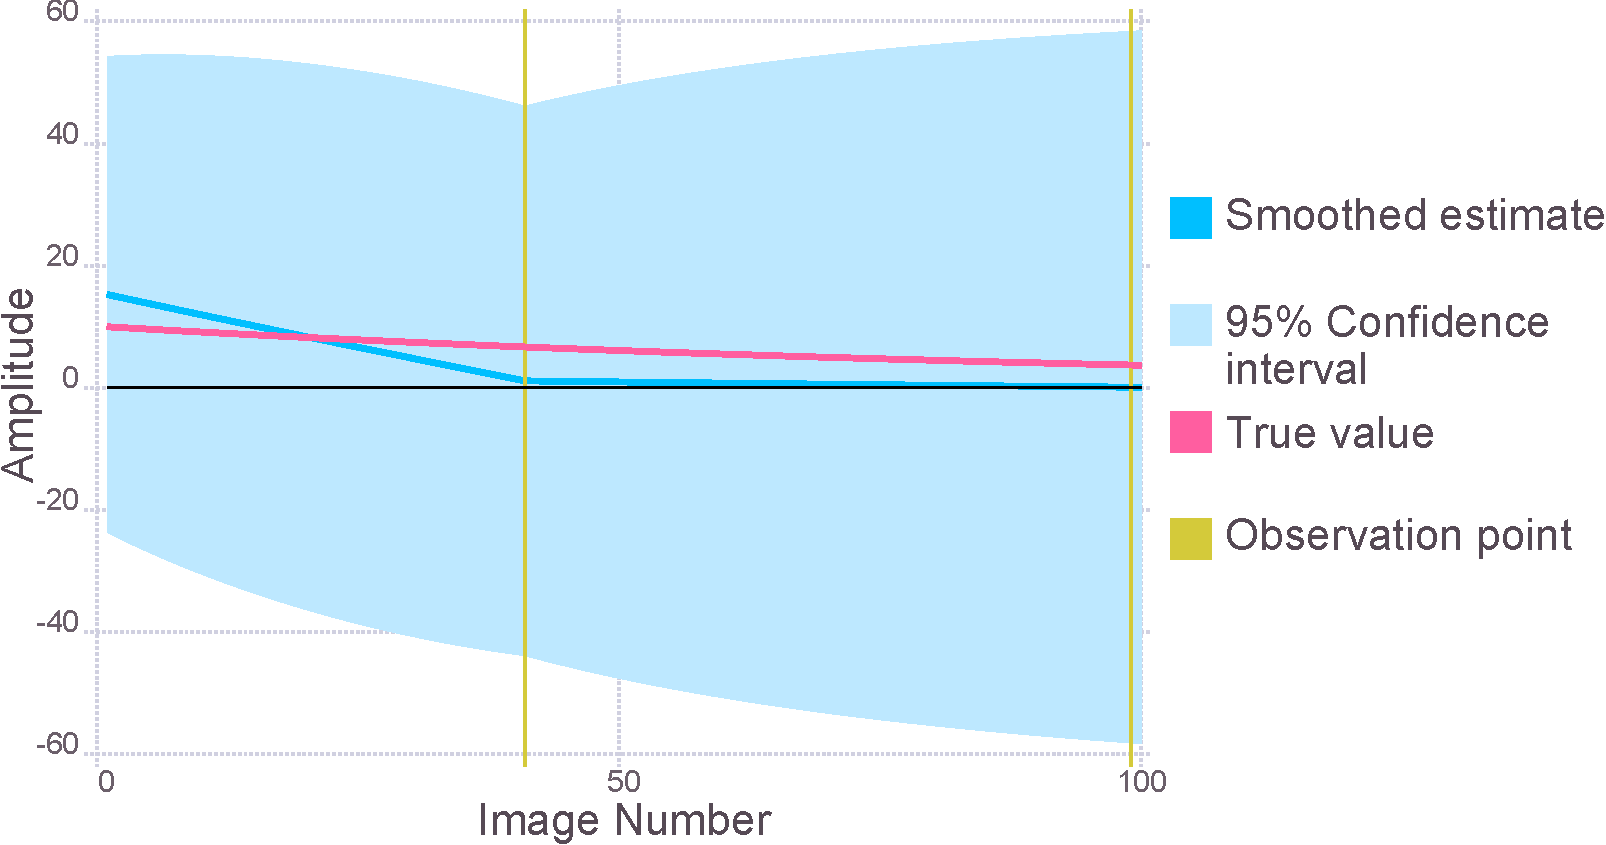
\includegraphics[width=\textwidth]{figures/datared/intDecSim1_bad.pdf}
        \caption{Cycle 1: backward pass.}
        \label{fig:URTSS simulation results - cycle 1 - bad}
    \end{subfigure}
\end{figure}
\begin{figure}
    \ContinuedFloat
    \begin{subfigure}[b]{1.0\textwidth}
        \centering
        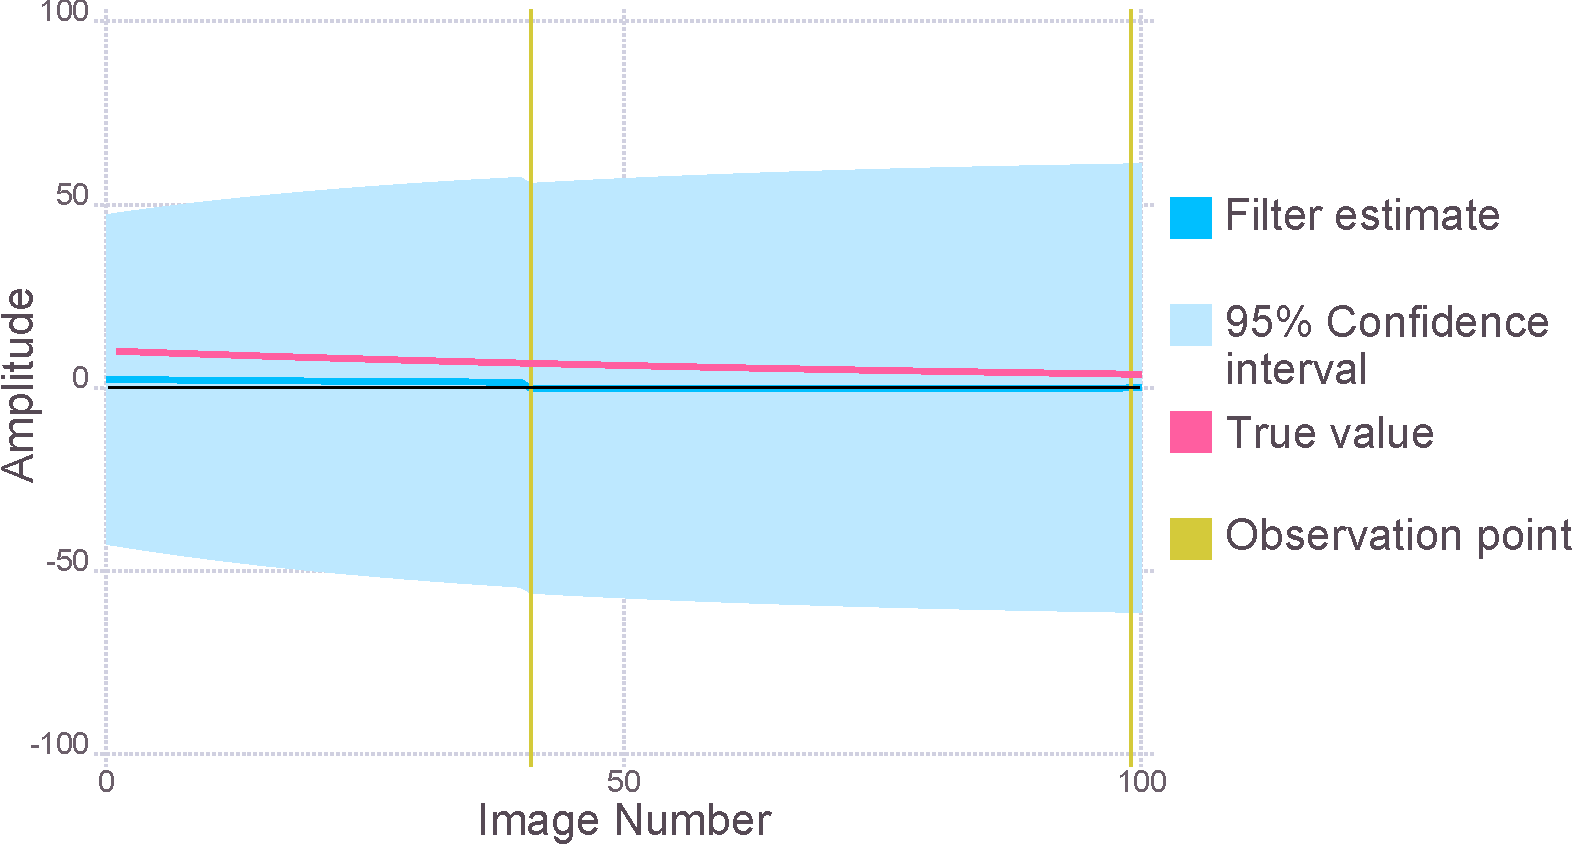
\includegraphics[width=\textwidth]{figures/datared/intDecSim_Filt8_bad.pdf}
        \caption{Cycle 8: forward pass.}
        \label{fig:UKF simulation results - cycle 8 - bad}
    \end{subfigure}
    \\
    \begin{subfigure}[b]{1.0\textwidth}
        \centering
        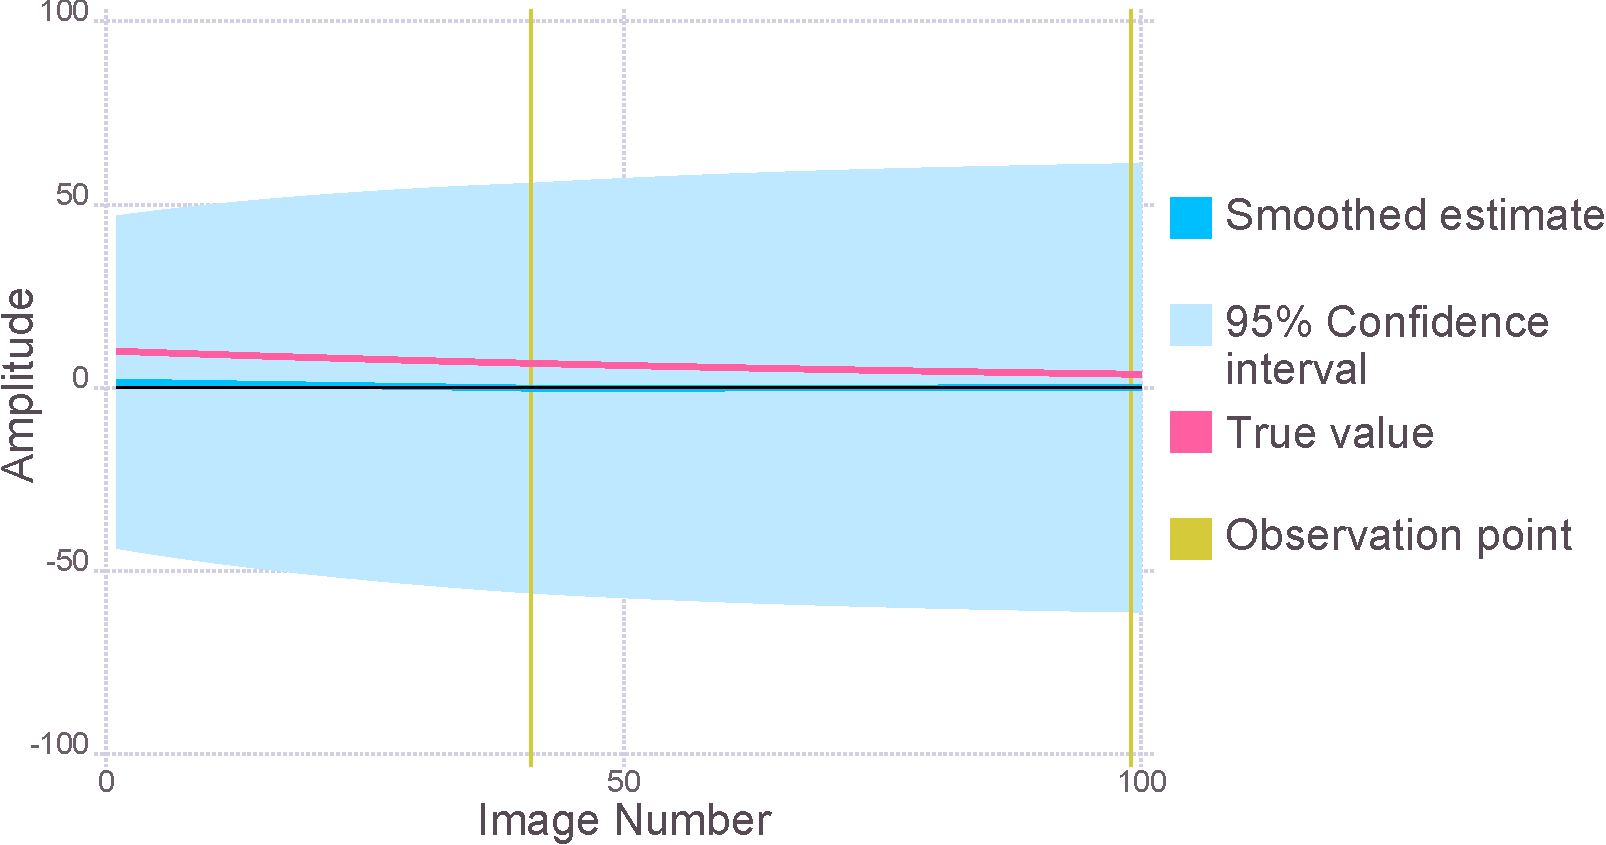
\includegraphics[width=\textwidth]{figures/datared/intDecSim8_bad.pdf}
        \caption{Cycle 8: backward pass.}
        \label{fig:URTSS simulation results - cycle 8 - bad}
    \end{subfigure}
    \caption{Forward-backward algorithm results for a simulated weak reflection observed on image 41 and 99 (solid gold lines) of a dataset consisting of 100 images.
    The forward-backward pass for cycle looks like it may lead to a good estimation of the true value.
    However, by cycle 8 the estimates have converged to zero and the 95\% confidence interval has not improved.}
    \label{fig:forward-backward algorithm simulation results - bad}
\end{figure}

The first cycle of the forward-backward algorithm looks promising as the estimate of the initial amplitude is slightly closer to the true value (Figure~\ref{fig:URTSS simulation results - cycle 1 - bad}).
However, at cycle 8 (Figure~\ref{fig:URTSS simulation results - cycle 8 - bad}) it is clear that the forward-backward algorithm is converging to a point where every amplitude estimate is zero, which is not representative of the true amplitude.
The log likelihood confirms that the estimates are getting worse as the values decrease with the cycle number (Figure~\ref{fig:Simulation Log likelihood - bad}).

\begin{figure}[ht!]
    \centering
    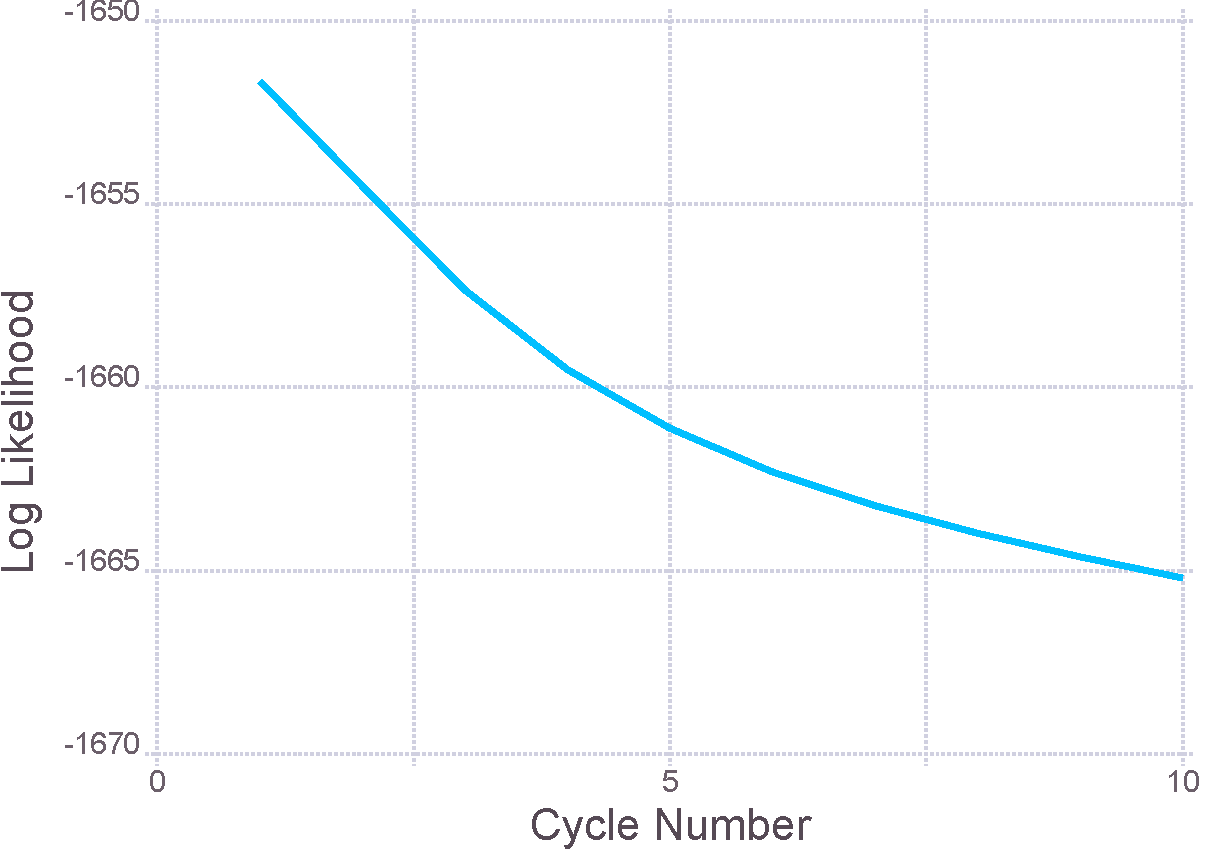
\includegraphics[width=1.0\textwidth]{figures/datared/loglik_bad.pdf}
    \caption{Log likelihood values calculated for each smoothing pass.
    Visually the forward-backward passes seemed to give worse estimates as the number of cycles increased (Figure~\ref{fig:forward-backward algorithm simulation results - bad}).
    The log likelihood values confirm this as evidenced by the decrease in the values.}
    \label{fig:Simulation Log likelihood - bad}
\end{figure}

To circumvent the problems caused by using the forward-backward algorithm on weak reflections, Bayesian inference is performed on the initial amplitude estimate at the end of each cycle.
In particular the expected value of the posterior distribution is used as the initial amplitude estimate.
The posterior distribution of interest is
\begin{equation}
	P(F_c | F_0) = \f{P(F_0 | F_c) \times P(F_c)}{P(F_0)},
	\label{eq:Baysian inference for weak reflections}
\end{equation}
where $P(F_0 | F_c)$ is defined for centric and acentric reflections as
\begin{align}
    &P_a(F_0 | F_c) = \f{2F_0}{\varepsilon \sigma_{0}^2} \exp \left(-\f{F_0^2 + \bs{D}^2F_c^2}{\varepsilon \sigma_{0}^2}\right)I_0 \left(\f{2F_0\bs{D}F_c}{\varepsilon \sigma_{0}^2}\right), \label{eq:Weak reflection likelihood function - acentric reflections} \\
    &P_c(F_0 | F_c) = \left[\f{2}{\pi \varepsilon \sigma_{0}^2}\right]^{1/2} \exp \left(-\f{F_0^2 + \bs{D}^2F_c^2}{2\varepsilon \sigma_{0}^2}\right) \cosh \left(\f{F_0\bs{D}F_c}{\varepsilon \sigma_{0}^2}\right), \label{eq:Weak reflection likelihood function - centric reflections}
\end{align}
and $P(F_c)$ is also defined for centric and acentric reflections as
\begin{align}
    &P_a(F_c) = \f{2F_c}{\Sigma^2} \exp \left(-\f{F_c^2}{\Sigma^2}\right), \label{eq:Weak reflection prior distribution - acentric reflections} \\
    &P_c(F_c) = \sqrt{\f{2}{\pi \Sigma^2}} \exp \left(-\f{F_c^2}{2\Sigma^2}\right), \label{eq:Weak reflection prior distribution - centric reflections}
\end{align}
where $P(F_c)$ is the Wilson distribution for amplitudes, $F_0$ and $\sigma_{0}^2$ are the initial amplitude and variance estimates from the forward-backward cycle and $F_c$ is the amplitude to be calculated.
As discussed in section \ref{sub:Probabilistic extrapolation}, the denominator of equation \ref{eq:Baysian inference for weak reflections} can be given as
\begin{equation}
	P(F_0) = \int_0^{\infty} P(F_0 | F_c) \times P(F_c)\, \mathrm{d}F_c.
\end{equation}
This procedure ensures that the initial amplitude value for the next forwards pass is positive.
If the final value for the amplitude at the end of a forwards pass is negative then that value is set to zero for the smoother.
Systematic testing is required to determine whether this is a robust solution to the problem 
